

\tikzset{every picture/.style={line width=0.75pt}} %set default line width to 0.75pt        

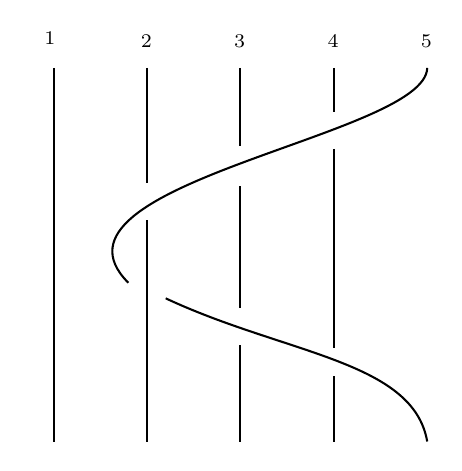
\begin{tikzpicture}[x=0.75pt,y=0.75pt,yscale=-1.5,xscale=1.5]
%uncomment if require: \path (0,877); %set diagram left start at 0, and has height of 877

%Straight Lines [id:da45747682112445587] 
\draw    (110,30) -- (110,150) ;
%Curve Lines [id:da780036391620541] 
\draw    (230,30) .. controls (229.5,52) and (102,67) .. (134,99) ;
%Straight Lines [id:da7231034545363801] 
\draw    (140,30) -- (140,67) ;
%Straight Lines [id:da42500416943536923] 
\draw    (140,79) -- (140,150) ;
%Curve Lines [id:da4654984332204606] 
\draw    (146,104) .. controls (184.5,122) and (225.5,124) .. (230,150) ;
%Straight Lines [id:da9660591521671449] 
\draw    (170,30) -- (170,55) ;
%Straight Lines [id:da38384623850853183] 
\draw    (170,68) -- (170,107) ;
%Straight Lines [id:da7201739522652382] 
\draw    (170,119) -- (170,150) ;
%Straight Lines [id:da2578634464595936] 
\draw    (200,56) -- (200,120) ;
%Straight Lines [id:da21734786864923916] 
\draw    (200,30) -- (200,44) ;
%Straight Lines [id:da1231057225472203] 
\draw    (200,129) -- (200,150) ;

% Text Node
\draw (106,17.4) node [anchor=north west][inner sep=0.75pt]  [font=\scriptsize]  {$1$};
% Text Node
\draw (137,18.4) node [anchor=north west][inner sep=0.75pt]  [font=\scriptsize]  {$2$};
% Text Node
\draw (167,18.4) node [anchor=north west][inner sep=0.75pt]  [font=\scriptsize]  {$3$};
% Text Node
\draw (197,18.4) node [anchor=north west][inner sep=0.75pt]  [font=\scriptsize]  {$4$};
% Text Node
\draw (227,18.4) node [anchor=north west][inner sep=0.75pt]  [font=\scriptsize]  {$5$};


\end{tikzpicture}